\documentclass[
  man,
  floatsintext,
  longtable,
  nolmodern,
  notxfonts,
  notimes,
  colorlinks=true,linkcolor=blue,citecolor=blue,urlcolor=blue]{apa7}

\usepackage{amsmath}
\usepackage{amssymb}




\RequirePackage{longtable}
% \setlength\LTleft{0pt}
\RequirePackage{threeparttablex}

% % 


\makeatletter
\renewcommand{\paragraph}{\@startsection{paragraph}{4}{\parindent}%
	{0\baselineskip \@plus 0.2ex \@minus 0.2ex}%
	{-.5em}%
	{\normalfont\normalsize\bfseries\typesectitle}}

\renewcommand{\subparagraph}[1]{\@startsection{subparagraph}{5}{0.5em}%
	{0\baselineskip \@plus 0.2ex \@minus 0.2ex}%
	{-\z@\relax}%
	{\normalfont\normalsize\bfseries\itshape\hspace{\parindent}{#1}\textit{\addperi}}{\relax}}
\makeatother




\usepackage{longtable, booktabs, multirow, multicol, colortbl, hhline, caption, array, float, xpatch}
\setcounter{topnumber}{2}
\setcounter{bottomnumber}{2}
\setcounter{totalnumber}{4}
\renewcommand{\topfraction}{0.85}
\renewcommand{\bottomfraction}{0.85}
\renewcommand{\textfraction}{0.15}
\renewcommand{\floatpagefraction}{0.7}

\usepackage{tcolorbox}
\tcbuselibrary{listings,theorems, breakable, skins}
\usepackage{fontawesome5}

\definecolor{quarto-callout-color}{HTML}{909090}
\definecolor{quarto-callout-note-color}{HTML}{0758E5}
\definecolor{quarto-callout-important-color}{HTML}{CC1914}
\definecolor{quarto-callout-warning-color}{HTML}{EB9113}
\definecolor{quarto-callout-tip-color}{HTML}{00A047}
\definecolor{quarto-callout-caution-color}{HTML}{FC5300}
\definecolor{quarto-callout-color-frame}{HTML}{ACACAC}
\definecolor{quarto-callout-note-color-frame}{HTML}{4582EC}
\definecolor{quarto-callout-important-color-frame}{HTML}{D9534F}
\definecolor{quarto-callout-warning-color-frame}{HTML}{F0AD4E}
\definecolor{quarto-callout-tip-color-frame}{HTML}{02B875}
\definecolor{quarto-callout-caution-color-frame}{HTML}{FD7E14}

\newlength\Oldarrayrulewidth
\newlength\Oldtabcolsep


\usepackage{hyperref}




\providecommand{\tightlist}{%
  \setlength{\itemsep}{0pt}\setlength{\parskip}{0pt}}
\usepackage{longtable,booktabs,array}
\usepackage{calc} % for calculating minipage widths
% Correct order of tables after \paragraph or \subparagraph
\usepackage{etoolbox}
\makeatletter
\patchcmd\longtable{\par}{\if@noskipsec\mbox{}\fi\par}{}{}
\makeatother
% Allow footnotes in longtable head/foot
\IfFileExists{footnotehyper.sty}{\usepackage{footnotehyper}}{\usepackage{footnote}}
\makesavenoteenv{longtable}

\usepackage{graphicx}
\makeatletter
\def\maxwidth{\ifdim\Gin@nat@width>\linewidth\linewidth\else\Gin@nat@width\fi}
\def\maxheight{\ifdim\Gin@nat@height>\textheight\textheight\else\Gin@nat@height\fi}
\makeatother
% Scale images if necessary, so that they will not overflow the page
% margins by default, and it is still possible to overwrite the defaults
% using explicit options in \includegraphics[width, height, ...]{}
\setkeys{Gin}{width=\maxwidth,height=\maxheight,keepaspectratio}
% Set default figure placement to htbp
\makeatletter
\def\fps@figure{htbp}
\makeatother


% definitions for citeproc citations
\NewDocumentCommand\citeproctext{}{}
\NewDocumentCommand\citeproc{mm}{%
  \begingroup\def\citeproctext{#2}\cite{#1}\endgroup}
\makeatletter
 % allow citations to break across lines
 \let\@cite@ofmt\@firstofone
 % avoid brackets around text for \cite:
 \def\@biblabel#1{}
 \def\@cite#1#2{{#1\if@tempswa , #2\fi}}
\makeatother
\newlength{\cslhangindent}
\setlength{\cslhangindent}{1.5em}
\newlength{\csllabelwidth}
\setlength{\csllabelwidth}{3em}
\newenvironment{CSLReferences}[2] % #1 hanging-indent, #2 entry-spacing
 {\begin{list}{}{%
  \setlength{\itemindent}{0pt}
  \setlength{\leftmargin}{0pt}
  \setlength{\parsep}{0pt}
  % turn on hanging indent if param 1 is 1
  \ifodd #1
   \setlength{\leftmargin}{\cslhangindent}
   \setlength{\itemindent}{-1\cslhangindent}
  \fi
  % set entry spacing
  \setlength{\itemsep}{#2\baselineskip}}}
 {\end{list}}
\usepackage{calc}
\newcommand{\CSLBlock}[1]{\hfill\break\parbox[t]{\linewidth}{\strut\ignorespaces#1\strut}}
\newcommand{\CSLLeftMargin}[1]{\parbox[t]{\csllabelwidth}{\strut#1\strut}}
\newcommand{\CSLRightInline}[1]{\parbox[t]{\linewidth - \csllabelwidth}{\strut#1\strut}}
\newcommand{\CSLIndent}[1]{\hspace{\cslhangindent}#1}





\usepackage{newtx}

\defaultfontfeatures{Scale=MatchLowercase}
\defaultfontfeatures[\rmfamily]{Ligatures=TeX,Scale=1}





\title{Contextual cuing survives an interruption from an endogenous cue
for attention}
\shorttitle{Contextual cuing and endogenous cuing}


\usepackage{etoolbox}








\authorsnames[{1},{1},{1},{1},{1},{2}]{Tom Beesley,Louise Earl,Hope
Butler,Inez Sharp,Ieva Jaceviciute,David Luque}







\authorsaffiliations{
{Lancaster University},{Universidad de Málaga}}






\leftheader{Beesley, Earl, Butler, Sharp, Jaceviciute and Luque}



\abstract{This document is a template.}
% 
\keywords{keyword1, keyword2, keyword3}

\authornote{\par{\addORCIDlink{Tom Beesley}{0000-0003-2836-2743}}
\par{ }
\par{       }
\par{Correspondence concerning this article should be addressed to Tom
Beesley, Lancaster University, Department of Psychology, Lancaster
University, UK, LA1 4YD, UK, Email: t.beesley@lancaster.ac.uk}
}


\makeatletter
\let\endoldlt\endlongtable
\def\endlongtable{
\hline
\endoldlt
}
\makeatother

\urlstyle{same}



% From https://tex.stackexchange.com/a/645996/211326
%%% apa7 doesn't want to add appendix section titles in the toc
%%% let's make it do it
\makeatletter
\xpatchcmd{\appendix}
  {\par}
  {\addcontentsline{toc}{section}{\@currentlabelname}\par}
  {}{}
\makeatother

\begin{document}

\maketitle


\setcounter{secnumdepth}{-\maxdimen} % remove section numbering

\setlength\LTleft{0pt}




blah blah Olson and Chun (2002)

blah blah (Olson \& Chun, 2002)

It is well established that the process of visual search is guided by
past experience. When we encounter a scene, the extent to which the
stimuli within that scene match representations in memory will determine
the effectiveness of the stimulus processing and subsequent search
through the scene. This cognitive process is studied in the lab using
the contextual cuing (CC) task: participants typically experience a
standard visual search task (i.e., serial processing; slow search), such
as searching for a T amongst L shapes. A set of search configurations is
repeated across trials, and response times to targets are faster
compared to those in configurations that do not repeat. Thus, the
repetition of the search configurations leads to the formation of a
representation of the configuration in memory, and future processing of
the same configuration activates this representation, driving more
efficient behaviour within that scene.

Much work has focused on the nature of the memory and attention
processes responsible for contextual cuing. The effect was initially
suggested to be implicit in nature, with repeated configurations
seemingly guiding search unconsciously: typically participants are
unable to articulate their knowledge of the repeated configurations, and
show poor ability to recognise learnt configurations in memory tests
(e.g., Chun \& Jiang, 1998; Colagiuri \& Livesey, 2016), although this
view of CC has been strongly contested (e.g., Smyth \& Shanks, 2008;
Vadillo et al., 2016). There are also a number of plausible
computational models of how memory representations of repeated
configurations are formed and result in the CC effect (e.g., Beesley et
al., 2015; Brady \& Chun, 2007). The predominant view is that the memory
representations are best characterised as associative in nature, whereby
distractors (or groups of distractors, see Beesley et al., 2016) form
associations that activate more strongly the contingent target position
within each repeated configuration.

The exact nature of how repeated configurations come to facilitate
visual search is the focus of much debate within the literature. Broadly
there are two quite distinct theoretical accounts of why responses are
faster for repeated configurations: the early attentional guidance
account, and the late response facilitation account. According to the
early account, recognition of the configuration leads to a more
efficient search process through the distractor array, such that the
target is localised (fixated) at an earlier time point in search.
Perhaps the clearest (and arguably simplest) evidence in support of this
account comes from studies of eye-tracking during CC. For example,
search through repeated configurations results in fewer fixations prior
to target localisation (e.g., Beesley et al., 2018; Tseng \& Li, 2004).
According to the late response facilitation account, the benefit for
repeated configurations comes about as a result of enhanced target
processing once it has been localised by attention. One
conceptualisation of this process is that repeated configurations lead
to a reduction in the evidence threshold required to ascertain that the
target is present in its location, such that responses can be initiated
earlier. Such an account has been put forward by Sewell et al. (2018),
in order to explain the evidence supporting the late account from
response time modelling of the CC effect.

It seems likely that the both early and late processes contribute to the
overall CC effect (for a review see Sisk et al., 2019). The current
article focuses on exploration of the early-stage attentional account of
CC. The term ``early'' here reflects the fact that the CC benefit is
present prior to the detection of the target and the initiation of the
response to the target. Analysis of eye-movements has shown that serial
visual search can be defined as having two distinct phases: an initial
ineffective search in which the direction of saccades is not consistent
(arguably random) and a secondary effective phase in which each saccade
will draw attention closer to the target. CC appears to result from
having more trials with a shorter ineffective phase.

One interpretation of these data is that CC is initially random, and
that the initial distractor processing is not beneficial for CC.
Supporting evidence for this account comes from Olson and Chun (2002),
where participants were trained on a CC task in which either all the
distractors repeated, those in the half of the screen containing the
target (short-range-context), or those in the half of the screen that
didn't contain the target (long-range-context). CC was observed in the
short-range-context, but not in the long-range-context condition. Thus
it would appear that the distractors further from the target are not
critical to the generation of a CC effect.

Brady and Chun (2007)'s computational account features a mechanism that
ensures spatial constraints are placed on the learning of associations
with relation to their proximity to the target. If the spatial
constraints are tuned to modulate learning and restrict associative
formations to only those distractors close to the target, this model can
accurately model the data from Olson and Chun (2002). Since the only
consequential mechanism in the model for CC is the associative weights
(and their modulation by spatial constraints), then one prediction that
follows from this account is that the initial phase of search is
inconsequential for observing CC.

The current article provides a test of this prediction by significantly
interrupting the search process with an endogenous cue for attention. In
all experiments participants complete a contextual cuing visual search
task but are also presented with an arrow that signals the side of the
screen on which the target will appear. Thus, this cue disrupts the
natural search process, eliminating entirely the early phase of search.
In contrast to the localised facilitation account, it's possible that
contextual cuing involves learning of a procedural template that guides
eye-movements in a consistent pattern for each repeated configuration.
While the initial process may be inefficient in nature, it may
nevertheless be an important part of the procedural response to the
configuration in terms of the sequence of eye-movements. Recent
experiments from (\textbf{seitz2023?})

\section{Transparency and Openness}\label{transparency-and-openness}

The raw data, analysis scripts, experimental materials, and the
manuscript source files, are available at
\url{http://github.com/tombeesley/CC_Control}. The analyses reported in
this manuscript are computationally reproducible from the manuscript
source files (using R v4.4.0), which are available at the github
repository. The study design and analyses were not pre-registered.

\section{Experiment 1}\label{experiment-1}

Experiment 1 sought to examine whether the learnt attentional behaviour
that develops during contextual cuing is expressed when participants are
directed by an endogenous (instructional) cue to search in a particular
region of the visual scene. Participants were first trained with a set
of four repeating configurations in phase 1 across 5 epochs of 32 trials
each. Then prior to phase 2, participants were told that an arrow would
appear before every trial indicating the side of the screen on which the
target would be located. This arrow was valid on every trial. In phase
2, the repeating configurations were presented in two forms:
``consistent'', where the target appeared in the same position as it has
appeared for that configuration in phase 1; and ``inconsistent'', where
the target appeared in a position in the opposite quadrant of the screen
from where it had appeared in phase 1. Random configurations were also
presented in this phase. If the contextual cues within the repeated
configurations continue to guide attention in the presence of the
instructional cue, then we would expect that response times would be
faster on consistent trials compared to random trials. In addition, we
would also expect that the contextual cues would guide attention
\emph{away} from the (new) target quadrant on inconsistent trials, and
so response times should be slower on these trials compared to those on
random trials.

\subsection{Method}\label{method}

\subsubsection{Participants}\label{participants}

Thirty-one undergraduate students from Lancaster University were
recruited (mean age = 20.1, SD = 1.1; 17 identified as female and 14 as
male) via the Psychology Research Participation System in the Department
of Psychology at Lancaster University, in return for the opportunity to
use the recruitment system for their own research in future years.

\subsubsection{Materials}\label{materials}

Participants were tested individually in a quiet room with a Dell laptop
with a 15.6'' screen, a screen resolution of 1920 x 1080, and a full
size external keyboard for participants to use to respond to the task.
Participants sat approximately 50 cm from the screen. Stimulus
presentation was controlled by MATLAB using the Psychophysics Toolbox
extensions (Brainard, 1997; Kleiner, Brainard \& Pelli, 2007; Pelli,
1997). Responses to the target stimulus were made by pressing the `c' or
`n' key on a standard keyboard. All experimental materials are available
at the github repository for this study.

Distractor stimuli were an `L' shape (rotated 0°, 90°, 180°, or 270°)
while the target stimulus was a `T' shape (rotated at either 90° or
270°). Stimuli were 8 mm square and arranged in a square grid of 144
evenly spaced cells (12 x 12) which was positioned centrally on the
screen and was 170 mm square. The grid itself was invisible to
participants. The fixation cross (displayed centrally before each trial)
was 4 mm square. The background of the screen was grey (RGB: .6, .6, .6)
and the stimuli were presented in black (RGB: 1, 1, 1). There was a
small offset in the vertical line of the `L' distractors, which
increased the similarity between the `L' distractors and the target `T',
making the search task more difficult (Duncan \& Humphreys, 1989).

\subsubsection{Design}\label{design}

Phase 1 employed a within-subjects design with factors of epoch (1-5)
and configuration (repeated and random). All configurations contained 16
distractors, equally divided between the four quadrants of the display,
and one target. Four repeated configurations were trained. Four target
locations were used, with one from each quadrant assigned to each of the
repeated configurations. These same four target positions were used for
the random configurations throughout the task. Each of these four target
positions was chosen at random from one of five locations within each
quadrant, that were approximately equidistant from the center of the
screen. Distractors could not appear in these target locations.

Phase 2 employed a within-subjects design with factors of epoch (6-10)
and configuration (repeated: consistent; repeated: inconsistent; random:
consistent; random:inconsistent). On each trial, there was a .5
probability that an ``inconsistent'' version of the configuration would
be presented. This meant that the target was relocated to a
diametrically opposed target position such as to maximise the
displacement from the trained target position (see
Figure~\ref{fig-schematic}). This could occur for both the repeated and
random configurations, hence creating four unique trial types for this
phase. While random configurations did not have a ``trained'',
associated, target position, it is necessary to divide the random trials
into consistent and inconsistent trial types in this way in order to
assess any target frequency effects that may occur, since the
inconsistent target locations used in this phase were novel.

\begin{figure}[H]

\centering{

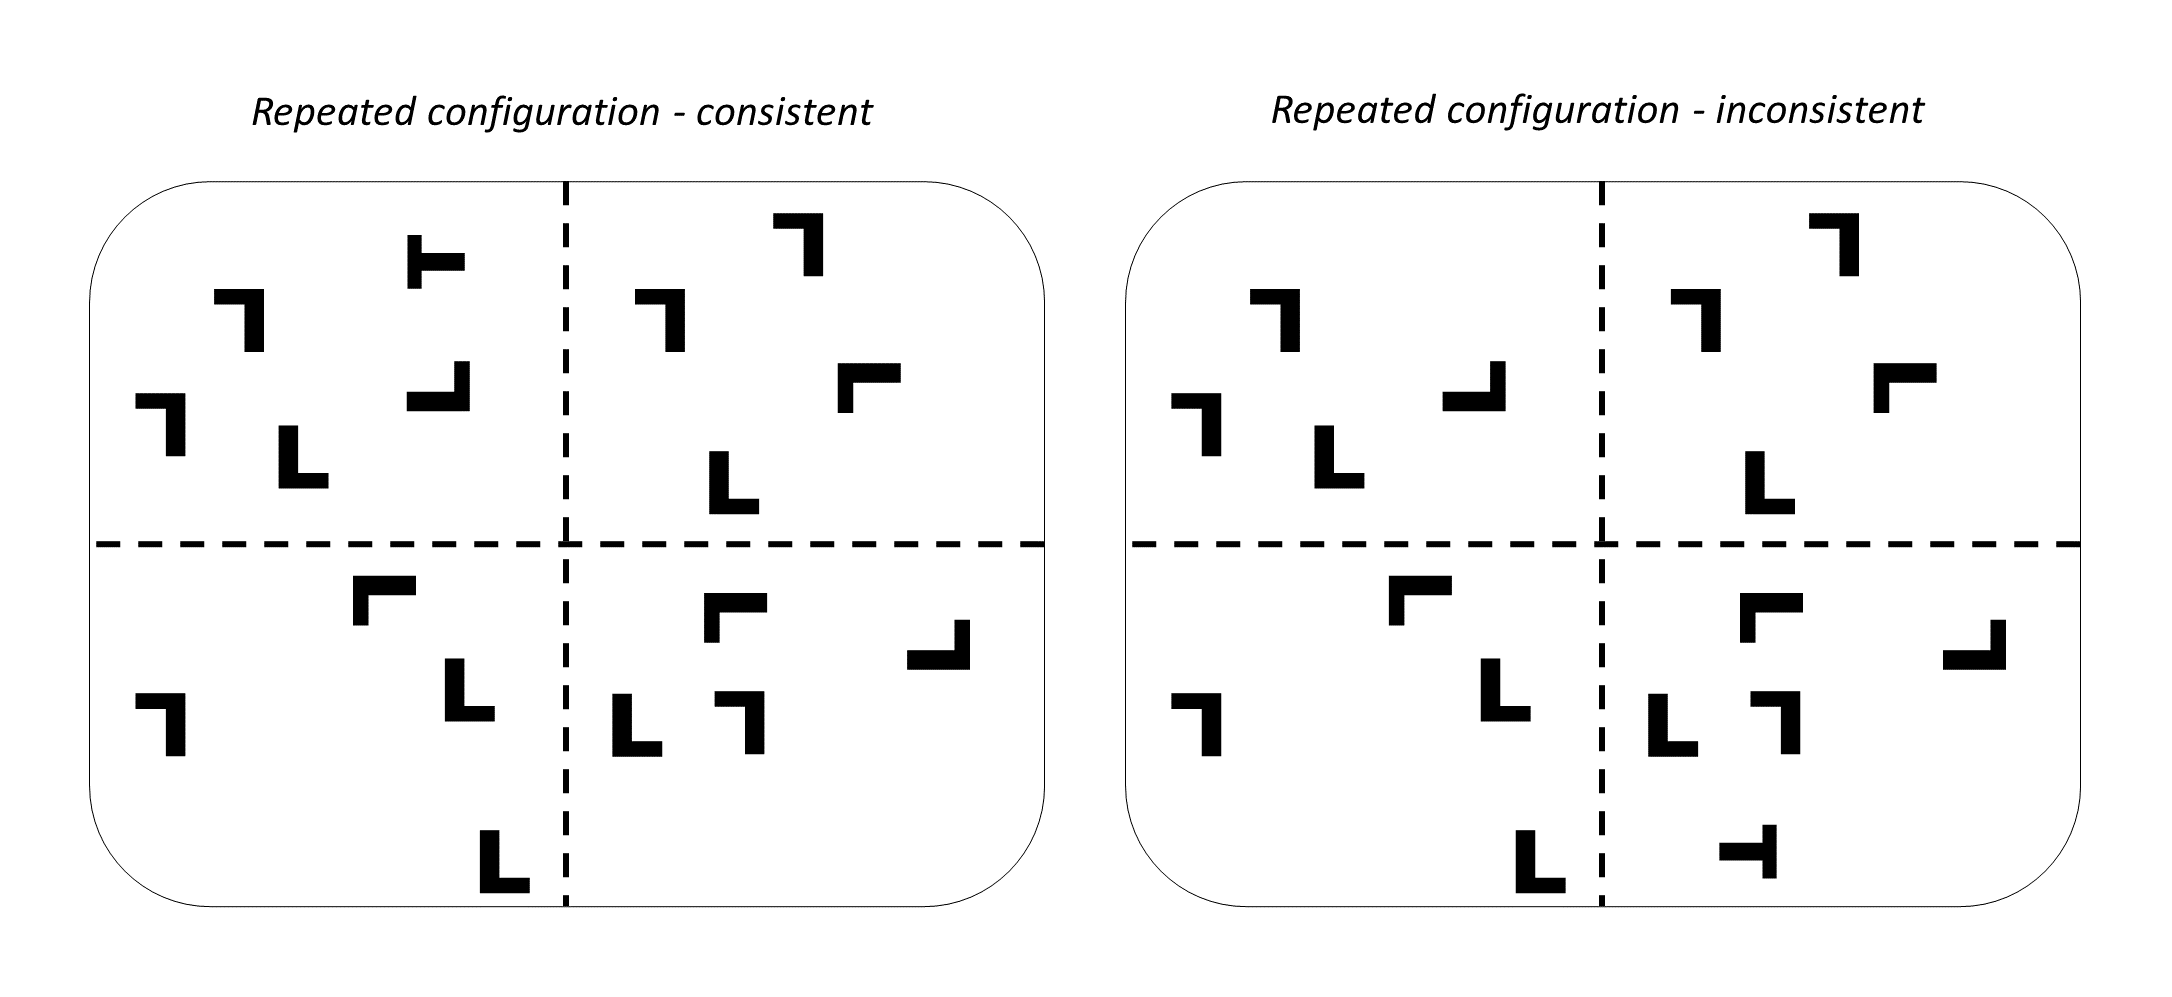
\includegraphics{Schematic.png}

}

\caption{\label{fig-schematic}Schematic of the manipulation of target
position in consistent and inconsistent trials of phase 2. The dashed
lines show the division of the stimuli into quadrants, but were not
present in the task procedure.}

\end{figure}%

\subsubsection{Procedure}\label{procedure}

Participants were tested individually in a quiet testing room. They were
given instructions on how to complete the task, including the
presentation of an example of a search trial. Participants were shown
the two correct responses for the two possible orientations of targets.

Each trial commenced with a fixation cross presented in the center of
the screen for 500 ms, which was then replaced immediately by the search
configuration. Participants searched for the target stimulus and
responded with a left or right response depending on its orientation.
Reaction times (RTs) were recorded from the onset of the search
configuration. Following a valid response (c or n), the configuration
was removed from the screen. The ITI was 1000 ms. If participants made
an incorrect response to the target orientation, ``INCORRECT RESPONSE''
appeared in red in the center of the screen for 3000 ms, prior to the
ITI. If participants did not respond within 6000 ms, ``TIMEOUT - TOO
SLOW'' appeared in red in the center of the screen for 3000 ms, prior to
the ITI.

Each block of eight trials contained each of the four different repeated
configurations and four random configurations. These eight
configurations could appear in any order with the constraint that the
position of the target did not repeat across trials or across
consecutive blocks.

A rest break of 30 seconds was given every 80 trials. Trials started
automatically after these breaks.

After 160 trials, prior to phase 2, participants were given an
instruction screen which detailed the arrow that would appear on the
screen prior to the configuration. They were able to ask any questions
they had at this stage and then proceeded to phase 2. The arrow appeared
for 1000ms following the fixation cross, before the presentation of the
search configuration. The task was otherwise identical to that used in
phase 1.

\subsection{Results}\label{results}

Our criterion for removing outlier data, at both the participant level
and the trial level, was 2.5 standard deviations above or below the mean
of the sample. On average, trials ended with a timeout on 1.97\% of
trials (SD = 2.53). Two participants had an usually high proportion of
timeouts and were removed from the analysis. The mean accuracy of
participants (not including timeout trials) was 98.10\% (SD = 1.65\%).
One participant had an unusually low proportion of accurate trials and
was also removed. The only participant deemed to be an outlier in terms
of mean response time (hereafter RT) was also excluded on the basis of
the timeout criterion, noted above.

For the remaining twenty-eight participants we removed trials with a
timeout and inaccurate trials, before removing outliers from the RT
data. On average, the proportion of outliers removed was 3.03\% (SD =
0.79\%). Zero participants had an unusual proportion of trials removed
as outlier RTs (greater than 2.5 SDs above the mean).

\begin{figure}[H]

\centering{

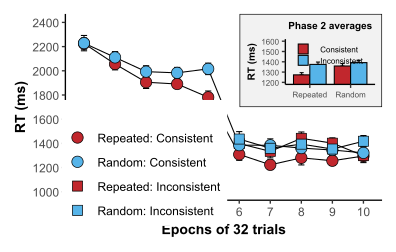
\includegraphics[width=0.9\textwidth,height=0.8\textheight]{CCEC_ms1_files/figure-pdf/fig-RT-exp1-1.pdf}

}

\caption{\label{fig-RT-exp1}RT data for Experiment 1. The phase 2
averages across the four trial types are shown inset. Within-subject
error bars were computed by a process of normalising the RT data for the
sample (\textbf{cousineau2005?}).}

\end{figure}%

Figure~\ref{fig-RT-exp1} shows the RT data across the 10 epochs of the
experiment. In phase 1 (epochs 1-5) a contextual cuing effect emerged,
with faster responses to repeated over random configurations. In phase
2, the presence of the guiding arrow led to a clear reduction in the
response times. For all participants, the mean RT across epochs 4 and 5
was higher than the mean RTs across epochs 6 and 7. Despite the clear
evidence for the processing of the endogenous cue, the underlying search
configuration continued to play a role in the guidance of attention,
with faster response times for (consistent) repeated configurations
compared to random configurations.

These data were analysed with a Bayesian ANOVA\footnote{The Bayesian
  analyses here follow the process outlined in Rouder et al. (2017).
  Briefly, we present the best fitting model evaluated against the null
  model, and then compare this fit to that of other models. Where the
  comparison of two models (i.e., A against B) reveals a Bayes Factor of
  greater than 3, this is taken as support for the components of model A
  that are not present in model B. Bayes Factors of less than 0.33 are
  taken as evidence in support of the equivalence of two models.
  Following Wetzels et al. (2011) we use the terms ``substantial''
  (BF\textgreater3; BF\textless1/3), and ``strong'' (BF\textgreater10;
  BF\textless1/10) to reflect the levels of support for the results of
  the model comparisons.}, using the \emph{BayesFactor::anovaBF()}
function in R. All analyses in this study used the default parameters
for the priors, which ``places mass in reason-able ranges {[}of effect
sizes{]} without being overcommitted to any one point'' (Rouder et al.,
2017, p. 317). First taking the data from phase 1 (epochs 1-5), there
was strong support for the model containing the factors of epoch and
configuration (repeated vs.~random), BF\textsubscript{10} = 2 ×
10\textsuperscript{12} ± 6.28\%. The addition of the interaction term
did not improve the model fit, BF = 0.52 ± 11.83\%, though there was no
evidence for the absence of the interaction. The best fitting model was
a better fit than the two models containing only one of the factors,
smallest BF = 31.64 ± 7.54\%, providing strong support for both the
effects of configuration and epoch. Partial eta-squared (\(n^2_p\))
effect sizes were calculated using \emph{effectsize::eta\_squared},
giving values of: 0.2169638 for the effect of configuration; 0.3897725
for the effect of epoch; and 0.1014833 for the interaction effect.

A Bayesian ANOVA on the data from phase 2 (epochs 6-10) found strong
support for the model containing the factors of configuration (repeated
vs.~random) and target position (consistent vs.~inconsistent),
BF\textsubscript{10} = 36.82 ± 8.34\%. The next best fitting model
contained these two factors and the interaction term, and was not a
substantially worse fit to the data, BF = 0.96 ± 29.79\%. The best
fitting model (with factors of configuration and target position, but no
interaction) was a substantially better fit to the data than the model
containing only the factor of configuration BF = 17.02 ± 10.9\%
providing evidence that RTs were faster on consistent than inconsistent
trials. There was no evidence for a difference between the best fitting
model and the model containing only the factor of target position, BF =
1.89 ± 12.93\%. The relevant effect sizes (\(n^2_p\)) were: 0.1394981
for the effect of configuration; 0.2230093 for the effect of target
position; and 0.1350565 for the interaction of these two factors.

To further explore responses to the different trial types in phase 2,
Bayesian t-tests were run using BayesFactor::ttestBF (using the default
Cauchy prior) for comparisons between the repeated and random
configurations, across the two target position conditions (consistent
and inconsistent). This revealed substantial support for a difference
between the response times on ``repeated: consistent'' trials and those
on the respective random trials (random: consistent),
BF\textsubscript{10} = 4.14 ± 0\%. There was also substantial evidence
to suggest there was no meaningful difference between the response times
for the ``repeated: inconsistent'' trials and the respective random
trials, BF\textsubscript{10} = 0.24 ± 0.03\%.

\subsection{Discussion}\label{discussion}

Experiment 1 sought to examine the consequence of an endogenous cue that
prompts top-down control of the search process on contextual cuing. In
phase 1 we established a robust contextual cuing effect. Following this,
participants received instruction that each trial would be preceded by
an arrow stimulus that would signal the side of the screen on which the
target would appear. This cue was valid on all trials in phase 2.
Consistent with these instructions and the processing of this cue, we
observed substantially reduced search times in phase 2 compared to phase
1. The same set of repeated configurations were presented in phase 2,
but for half of the trials, the target was relocated to the diagonally
opposed quadrant of the screen. Therefore, on these ``repeated
inconsistent'' trials, the underlying configuration of distractors
predicted the target in a location that opposed that of the (valid)
endogenous cue. Across this phase we observed significant contextual
cuing for the repeated consistent trials, demonstrating that the
underlying configuration of distractors continued to guide attention in
the presence of the endogenous cue. However, the repeated inconsistent
trials did not lead to an impairment in response times relative to
random trials, suggesting that the underlying configuration did not
influence search on these trials.

\section{Experiment 2}\label{experiment-2}

In Experiment 1 we demonstrated that an established effect of contextual
cuing is maintained even when attention is being guided by the presence
of a valid endogenous cue. That is, we found that the \emph{performance}
of an established search behaviour in contextual cuing is not disrupted
by concurrent top-down goals to guide attention in a controlled manner.
In Experiment 2 we wanted to explore whether the \emph{learning} of the
contextual cue itself was affected by the presence of a valid endogenous
cue. That is, does the presence of a valid endongenous cue, which leads
to a controlled command of attention, limit the development of a
contextual cuing effect. To do this, we trained each participant on two
sets of repeating configurations. One of these sets was always presented
in the presence of a valid endogenous cue, while the other set was
always presented in the absence of the endogenous cue. The extent to
which there is a ``cue-competition'' effect between the endogenous cue
and the contextual cues can be examined by comparing the contextual
cuing effect we observe for the two sets of configurations. Given the
clear difference in RTs we observed in Experiment 1 between the trials
with the endogenous cue present and the cue being absent, we anticipated
the same difference in responding in Experiment 2. Therefore we also
included a second phase of Experiment 2 in which we removed the
endogenous cue entirely from the task. This second phase therefore
allowed us to directly compare the contextual cuing for the two sets of
configurations when RTs were at a comparable level.

``Cue-competition'' effects have been examined previously in contextual
cuing. Endo and Takeda (2004) trained participants with a contextual
cuing task composed of distractor location configurations and repeating
distractor identities. Their experiments suggested that the stronger
configural (spatial) cue out-competed the cue provided by the distractor
identities. Similarly, Kunar et al. (2014) found that when colour cues
and configural cues both predicted the target location, configural cues
were dominant and tended to overshadow the weaker colour cue. Beesley
and Shanks (2012) looked at the cue-interaction effects \emph{within} a
configuration of distractors. Participants were first trained with half
a configuration of repeating distractors that predicted the target (8
out of 16 distractors). In a later stage these distractors were paired
with a new half-configuration, such that the whole configuration now
predicted the same target location. In contrast to the predictions of
the vast majority of models of contingency learning, learning about
these new predictive distractors was facilitated, rather than impaired
in this second phase (relative to a control condition). Thus, Beesley
and Shanks (2012) found that cue-competition was not observed within a
configuration of equally predictive distractors. Together these studies
suggest that the spatial configuration serves as a strong cue for the
target and will out-compete non-configural cues for access to the
learning mechanism. The dominance of the configuration in these
situations may therefore lead to the prediction that the endogenous cue
would not ``block'' the learning of the configuration in the current
task.

\subsection{Method}\label{method-1}

\subsubsection{Participants}\label{participants-1}

Thirty-four undergraduate students from Lancaster University were
recruited (mean age = 20.7352941, SD = 5.2932709; 28 identified as
female and 6 as male) via the Psychology Research Participation System
in the Department of Psychology at Lancaster University, in return for
the opportunity to use the recruitment system for their own research in
future years.

\subsubsection{Materials}\label{materials-1}

Participants were tested in a quiet laboratory testing cubicle, with a
standard PC and a 24'' monitor set at a resolution of 1920 x 1080
pixels. Since the monitor was larger for this experiment, the dimensions
of the presented stimuli had a proportional increase in size: Distractor
stimuli were 11 mm square; the search grid was 240 mm square; the
fixation cross was 6 mm square. In all other respects, the materials
were the same as those detailed in Experiment 1.

\subsubsection{Design}\label{design-1}

Four repeated configurations were created in an identical manner to
those used in Experiment 1. For each participant, two of these
configurations were used for the ``cue-competition'' condition, in which
the arrow cue was presented before the configuration, while two were
used for the ``control'' condition (no arrow presented). As in
Experiment 1, the four repeated configurations were paired with unique
target positions from each of the four quadrants. We counterbalanced the
use of the target quadrants across the factors of configuration type
(repeated and random) and cue condition (cue-competition and control).
For half of the participants, targets in the top left and bottom right
were used for the repeated configurations presented with the arrow
(cue-competition) condition, with targets in the top right and bottom
left used for repeated configurations in the no-arrow (control)
condition. For these participants, random configurations presented with
the arrow had targets in the top right and bottom left, and random
configurations without the arrow had targets in the top left and bottom
right. For the other half of the participants these assignments were
reversed (repeated-arrow: top-right and bottom-left; repeated-no arrow:
top-left and bottom-right; random-arrow: top-left and bottom-right;
random-no arrow: top-right and bottom-left).

\subsubsection{Procedure}\label{procedure-1}

The procedure was the same as Experiment 1 with the following
differences. Participants received 320 trials in total. For the first
160 trials, the arrow was presented for the relevant conditions. For the
final 160 trials, the arrow was never presented. Rest breaks were given
every 60 trials.

\subsection{Results}\label{results-1}

Our criteria for removing outlier data were identical to Experiment 1.
On average, trials ended with a timeout on 2.13\% of trials (SD = 1.83).
Zero participants had an usually high proportion of timeouts. The mean
accuracy of participants (not including timeout trials) was 95.85\% (SD
= 6.10\%). One participant had an unusually low proportion of accurate
trials and were removed from the sample. Zero participants were deemed
to be an outlier in terms of mean RT.

For the remaining thirty-three participants we removed trials with a
timeout and inaccurate trials, before removing outliers from the RT
data. On average, the proportion of outliers removed was 2.81\% (SD =
1.04\%). One participant had an unusual proportion of trials removed as
outlier RTs and were not included in the final analysis.

\begin{figure}[H]

\caption{\label{fig-RT-exp2}RT data for Experiment 2. Error bars show
standard error of the mean on normalised data.}

\centering{

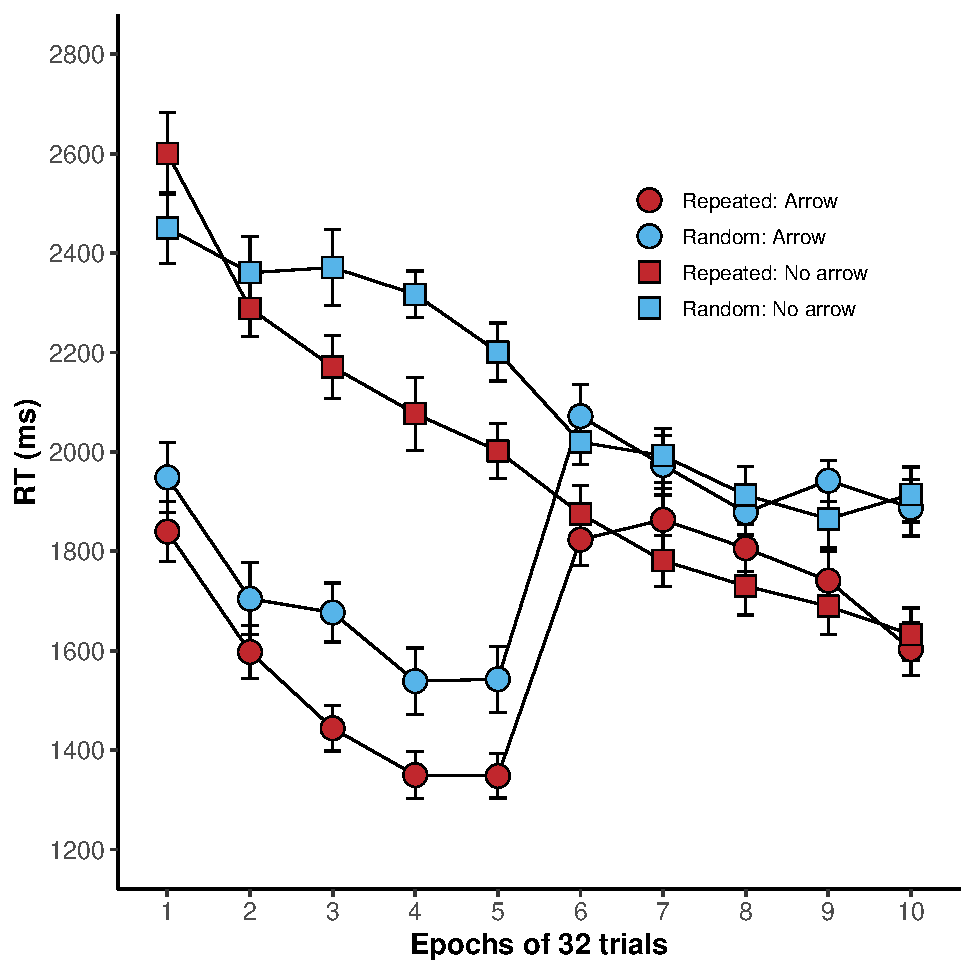
\includegraphics[width=0.8\textwidth,height=0.8\textheight]{CCEC_ms1_files/figure-pdf/fig-RT-exp2-1.pdf}

}

\end{figure}%

Figure~\ref{fig-RT-exp2} shows the RT data across the 10 epochs of the
experiment. Contextual cuing emerged rapidly in both the arrow and
no-arrow conditions, with little suggestion that the CC effect was
different in the two conditions. The phase 1 data were explored with a
Bayesian ANOVA, which revealed that the best fitting model contained the
factors of epoch, configuration (repeated vs.~random), and endogenous
cue (arrow present vs.~arrow absent), with no interaction terms,
BF\textsubscript{10} = 7.4 × 10\textsuperscript{100} ± 31.31\%. The next
best fitting model contained all three factors and the interaction of
epoch and configuration, BF\textsubscript{10} = 5.8 ×
10\textsuperscript{100} ± 15.4\%, and this model was not a substantially
worse fit to the data, BF = 0.79 ± 34.89\%. All other models were
substantially worse fits than the best fitting model, largest BF = 0.17
± 19.95\%. Importantly, the interaction term between the factors of
endogenous cue and configuration did not improve the fit of the model,
providing substantial support for the absence of this interaction, BF =
0.13 ± 33.78\%. The relevant effect sizes (\(n^2_p\)) were: 0.018597 for
the effect of epoch; 0.3973327 for the effect of configuration;
0.8454521 for the effect of endogenous cue; 0.1240887 for the
interaction effect between configuration and epoch; and 0.0227117 for
the interaction between configuration and endogenous cue.

When the endogenous cue was removed in the second half of the
experiment, RTs were equivalent across the two conditions. An effect of
configuration was seen for both cuing conditions, with little
discernible difference between the size of the cuing effects. We
conducted a Bayesian ANOVA with factors of epoch, configuration and
endogenous cue condition (arrow vs.~no-arrow). The best fitting model
was that with just the factors of epoch and configuration with no
interaction between the factors, BF\textsubscript{10} = 8.2 ×
10\textsuperscript{14} ± 4.79\%. There was substantial support for this
model over the next best fitting model, BF = 6.82 ± 20.71\%. To examine
the interaction of the configuration and endogenous cue factors, we
compared the model containing those two factors to the model containing
the two factors plus the interaction of configuration and endogenous
cue, which revealed substantial support for the absence of an
interaction, BF = 0.11 ± 13.77\%. The relevant effect sizes (\(n^2_p\))
were: 0.6153937 for the effect of configuration; and 0.2521965 for the
effect of epoch.

To provide further support for the absence of the interaction between
the factors of configuration type and endogenous cue, the data from
across the experiment (epochs 1-10) were analysed with a Bayesian ANOVA
with only the factors of configuration and endogenous cue. The best
fitting model was that with the two factors and no interaction,
BF\textsubscript{10} = 3.4 × 10\textsuperscript{51} ± 9.68\%. The
addition of the interaction term did not strengthen the model, with
substantial evidence for the absence of the interaction, BF = 0.07 ±
12.28\%. The relevant effect sizes (\(n^2_p\)) were: 0.7699908 for the
effect of the endogenous cue; and 0.606466 for the effect of
configuration.

\subsection{Discussion}\label{discussion-1}

Experiment 2 sought to examine whether the presence of a valid
endogenous cue would impair the acquisition of a contextual cuing
effect. In the first phase, two sets of configurations were trained, one
of which was always presented in the presence of the endogenous cue, and
one set which was presented without the endogenous cue. Overall there
was considerable evidence that the cue was processed and acted upon, as
response times to the target were much faster on cued trials. However,
there was no evidence to suggest that this initial guidance of attention
impaired the acquisition of the configurations on those trials.
Furthermore, when the endogenous cue was never presented in the final
phase of the experiment, the size of the contextual cuing effect was
equivalent between the two sets of configurations; the Bayesian analyses
found support for the equivalence of these CC effects.

The lack of competition effects seen in Experiment 2 are at odds with
some findings in the CC literature (i.e., Endo \& Takeda, 2004; Kunar et
al., 2014), where competition has been seen by more dominant or salient
features of the displays. Instead, the findings point towards a more
automatic nature to contextual cuing, whereby associations form
ubiquitously, so long as they receive the focus of attention at some
point within the search process (e.g., Beesley \& Shanks, 2012).

Taken together with the findings of Experiment 1, these data suggest
that when attention is cued in an endogenous manner, the underlying
search configuration will still play a significant role in guiding
search for the target. Since the endogenous cue appears at the point of
fixation, the most plausible interaction of these processes is that the
guidance by the endogenous cue is followed by the guidance by the
repeated context. The equivalence of the CC effects in the two
conditions (cued and uncued) would therefore suggest that the guidance
by the context was driven largely (or perhaps entirely) by the
distractors that appear close to the target. Accordingly, the longer
search times in the uncued condition suggest that more distractors are
processed in this condition, but that the influence of the repeated
distractors on attentional guidance may be limited to those occurring
later in the search process, and therefore those nearer to the target.
Alternatively, the interaction of these two processes (endogenous and
configuration-driven attention) need not interact in this order. It is
at least possible that the configuration is processed rapidly at the
onset of the trial, before the effects of the endogenous cue on
attention are observed. If this is the case, then those repeated
distractors that influence search (producing the CC effect) need not be
localised around the target. Experiment 3 provided a test of these two
possible accounts.

\section{Experiment 3}\label{experiment-3}

Existing data from studies of contextual cuing has pointed towards a
localised learning effect for repeated configurations, with those
distractors closest to the target being preferentially weighted in the
learning process over those located further from the target. For
example, Olson and Chun (2002) trained participants with three sets of
repeating configurations that differed in terms of which distractors
repeated across trials. For one set, the entire global context (all of
the distractors) repeated, while for the other two sets only the
short-range (those close to the target) or the long-range distractors
(those far from the target) repeated across trials. They found no
difference between the CC effect in the short-range and global
configurations, while the CC effect was not significant for the
long-range context. Similar results have been shown by Brady and Chun
(2007) which led to the development of the spatial constraints model of
contextual cuing, in which distractor-target associations occurring in
close proximal space are weighted more heavily in the learning process
(over those occurring across greater spatial distance).

It is important to consider how the bias towards local learning may
interact with the attentional scanning process during contextual cuing.
The analysis of eye-movements during contextual cuing tasks (Beesley et
al., 2018; Tseng \& Li, 2004) has revealed a characteristic scanning
pattern comprising two phases: search initially occurs in a seemingly
random manner, as the eyes move between distractors in the central
region of the distractor field, before then moving in a more directed
manner towards the target position. Contextual cuing appears to result
from a cessation of the first (random) search phase at an earlier time
point in the entire search process, such that processing of repeated
distractors will, on average, result in fewer fixations. With respect to
the current study, in Experiments 1 and 2 we have initially directed
attention towards the side of the screen that contains the target on
cued trials. This may bring about an early cessation of the first phase
of the search process. From here, however, it seems that search is still
facilitated by the repetition of the context.

To test this characterisation of the interaction between the endogenous
cue and the repeated context, we exposed participants to the same
procedure as used in phase 1 of Experiment 1, which establishes a
contextual cuing effect prior to the use of the endogenous cue. In a
second phase we then presented the endogenous cue on every trial (as in
Experiment 1), but we manipulated the presence of the repeated
distractors within the configurations. For each repeated configuration
we created two variations: in the ``proximal'' configurations, only the
distractors in the quadrant containing the target match those from the
full repeated configuration, while the distractors in the other three
quadrants were randomly arranged on each trial; in the ``distal''
configurations, the distractors closest to the target were randomised,
while the distractors in the other three quadrants were the same as
those in the full repeated configuration. During this phase we also
presented fully repeated configurations and fully randomised
configurations. Comparison of the response times across these four trial
types will allow us to determine the contribution of proximal and distal
distractors to the CC effect when attention is cued endogenously.

\subsection{Method}\label{method-2}

\subsubsection{Participants}\label{participants-2}

Forty-two undergraduate students from Lancaster University were
recruited (mean age = 18.6428571, SD = 2.8440904; 28 identified as
female and 14 as male) via the Psychology Research Participation System
in the Department of Psychology at Lancaster University, in return for
the opportunity to use the recruitment system for their own research in
future years.

\subsubsection{Materials}\label{materials-2}

All materials, including stimuli and testing environment were identical
to Experiment 2.

\subsubsection{Design}\label{design-2}

The design of phase 1 was identical to Experiment 1, with four repeated
configurations created and presented with random configurations during
this phase. For phase 2, each of the four configurations was manipulated
to create two alternative conditions. In the ``Repeated distal''
condition, the four distractors in the target quadrant were randomly
arranged on each trial, while the 12 distractors in the other three
quadrants were presented in the same positions as had been trained in
phase 1. Thus, slower response times for this condition (compared to the
fully repeated configurations) would indicate the extent to which
participants CC was governed by the distractors closest to the target.
For the ``Repeated proximal'' condition, the four distractors in the
target quadrant were presented in the same positions as had been trained
in phase 1, while the 12 distractors in the other three quadrants were
randomly arranged on each trial. Thus, slower response times for this
condition (compared to the fully repeated configurations) would indicate
the extent to which CC was governed by the distractors further from the
target. Comparison of the RTs for these different configurations with
those of the random configurations would allow for the assessment of
whether these subsets of distractors had \emph{any} contribution to the
CC effect that had developed during phase 1.

\subsubsection{Procedure}\label{procedure-2}

The procedure was identical to Experiment 1.

\subsection{Results}\label{results-2}

Our criteria for removing outlier data were identical to Experiment 1.
On average, trials ended with a timeout on 2.81\% (SD = 2.25) of trials
. Two participants had an usually high proportion of timeouts and were
removed from the sample. The mean accuracy of participants (not
including timeout trials) was 96.09\% (SD = 8.57\%). Two participants
that had an unusually low proportion of accurate trials and were also
removed. Zero participants were deemed to be an outlier in terms of mean
RT.

For the remaining thirty-eight participants we removed trials with a
timeout and inaccurate trials, before removing outliers from the RT
data. On average, the proportion of outliers removed was 3.17\% (SD =
0.71\%). Zero participants had an unusual proportion of trials removed
as outlier RTs.

\begin{figure}[H]

\caption{\label{fig-RT-exp3}RT data for Experiment 3. Error bars show
standard error of the mean on normalised data.}

\centering{

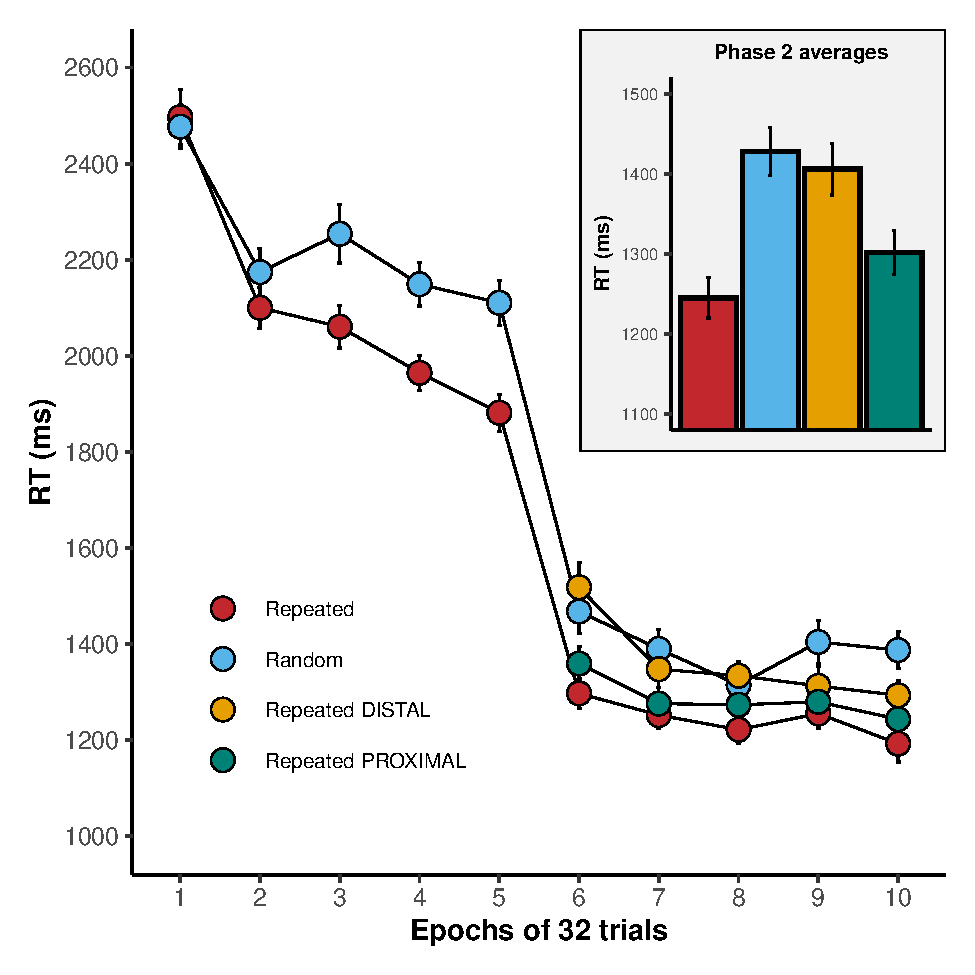
\includegraphics[width=0.8\textwidth,height=0.8\textheight]{CCEC_ms1_files/figure-pdf/fig-RT-exp3-1.pdf}

}

\end{figure}%

Figure~\ref{fig-RT-exp3} (main panel) shows the RT data across the 10
epochs of Experiment 3. As in Experiment 1, contextual cuing was readily
established in phase 1. These data were subjected to a Bayesian ANOVA
which revealed that the best fitting model contained the factors of
configuration (repeated vs.~random) and epoch, and an interaction
between those factors, BF\textsubscript{10} = 5.1 ×
10\textsuperscript{24} ± 10.67\%. However, the model without the
interaction provided a strong fit to the data, BF\textsubscript{10} =
5.2 × 10\textsuperscript{24} ± 10.3\%, and a comparison between the two
models did not find any evidence in support of the interaction term, BF
= 1.01 ± 14.83\%. There was strong support for the best fitting model
over the remaining models, smallest BF = 3957.7 ± 10.92\%, providing
strong support for the factors of epoch and configuration. The relevant
effect sizes (\(n^2_p\)) were: 0.3790593 for the effect of the
endogenous cue; and 0.4687663 for the effect of configuration; and
0.0805809 for the interaction of these two factors.

The response times decreased significantly with the presentation of the
valid endogenous cue in phase 2. Response times to the fully repeated
configurations were somewhat comparable to those when just the proximal
repeated distractors were present. Response times for the distal
repeated distractors appeared to be slower and comparable to the fully
random configurations. The phase 2 data were subjected to a Bayesian
ANOVA which found that the best fitting model contained the factors of
configuration and epoch but no interaction between the factors,
BF\textsubscript{10} = 1.3 × 10\textsuperscript{14} ± 5.98\%. This model
provided a superior fit to the data compared to the next best fitting
model that included the two factors and the interaction term, BF =
125.35 ± 7.96\%, providing strong support for the contribution of the
two factors and the absence of an interaction between the two factors.
The relevant effect sizes (\(n^2_p\)) were: 0.3722881 for the effect of
configuration; and 0.159434 for the effect of epoch.

The inset graph in Figure Figure~\ref{fig-RT-exp3} shows the mean RTs to
the four types of configuration, averaged across the 5 epochs of phase
2. To explore the differences in response times, Bayesian t-tests were
run for all pairwise comparisons. The response times to repeated and
repeated-proximal configurations were both faster than those to random
configurations, smallest BF\textsubscript{10} = 10313.81 ± 0\%. In
contrast, there was no evidence that the response times to
repeated-distal configurations were different from those to random
configurations, BF\textsubscript{10} = 0.39 ± 0.04\%. Response times to
repeated configurations were faster than those to repeated-proximal
configurations, BF\textsubscript{10} = 4.67 ± 0\%. Response times to
repeated-proximal configurations were faster than those to
repeated-distal configurations, BF\textsubscript{10} = 31.88 ± 0\%.

\subsection{Discussion}\label{discussion-2}

Experiment 3 explored the localisation of the distractors driving
contextual cuing when attention is guided by an endogenous cue. As
expected, there was substantial evidence that contextual cuing was
present when the distractors close to the target were maintained, but
not when these distractors were randomly arranged. These data suggest a
particular order to the interplay between the two drivers of attention:
initially attention is guided by the endogenous cue towards one half of
the screen, and then search is refined by the presence of the valid
configural cues (the repeated distractors). Like in Experiment 1, the
phase 2 data demonstrate the resilience of the CC effect to changes in
the search process. Despite visual search never commencing in a cued
manner during the initial acquisition period of phase 1, a CC effect was
readily observed in phase 2. Thus it seems that the stored
representations of configurations surrounding target positions are very
flexibly deployed in visual search. Notably the fully repeated
configurations exerted more of a benefit on search than those containing
only the proximal distractors, suggesting that the repeating distractors
beyond the target quadrant have some (but possibly lesser) influence on
search (Brady \& Chun, 2007).

These data lend support to the notion that the effect of the repeated
configuration is a late process within visual search, and that each
trial commences with a random search process that is not guided by the
repeated configuration (Beesley et al., 2018; Tseng \& Li, 2004). In
some ways, these findings represent a paradox of CC: the cuing effect
occurs almost at the point at which target detection has been made. One
interpretation would be that this exemplifies the role of spatial
contiguity in the formation of visual associations (Renaux et al.,
2017). Alternatively, it provides support for the proposed ``decision
threshold'' accounts of CC (Kunar et al., 2007; Sewell et al., 2018),
which posit that the repeated distractors close to the target ensure a
reduced threshold for target detection, resulting in faster response
times.

\section{General Discussion}\label{general-discussion}

Three experiments explored the impact of a central endogenous cue on the
contextual cuing of visual search. In Experiment 1, having established a
contextual cuing effect, each trial was preceded by an central
endogenous cue of attention in the form of an arrow, directing attention
towards the side of the screen in which the target was positioned (this
arrow cue was always valid in each of the three experiments). Despite
participants clearly using this cue, visual search was still facilitated
by the presence of the repeating pattern of visual search. This
experiment demonstrated that, once acquired, the activation of the
memory representation and its impact on performance of visual search
remains intact in the presence of a top-down instruction to guide
attention. Experiment 2 examined the storage of these contextual
representations, and whether these were impaired by an endogenous cue
guiding search. We found equivalent levels of contextual cuing for two
sets of configurations, one of which was paired with the cue and one
which was not. Together, these two experiments suggest a seamless
interplay between these two factors governing attention in visual
search: the endogenous cue initially guides attention and the repeated
configuration continues to refine and guide attention towards a fixation
on the target. In Experiment 3 we therefore explored whether the
localised distractors around the target were sufficient to generate CC
following the guidance by the endogenous cue. Indeed, there was a
significant CC effect in the case of the proximal distractors, albeit
slightly weaker than that generated by the entire repeated
configuration. Importantly, those repeated configurations that did not
contain the proximal distractors failed to generate a CC effect,
suggesting that the proximal distractors play a crucial role in search
following the guidance of attention by the endogenous cue.

The effect of CC on visual search has frequently been characterised as
an automatic influence on behaviour (e.g., Chun \& Jiang, 1998; Chun \&
Nakayama, 2000; Geyer et al., 2021). This characterisation of CC comes
from multiple aspects of the observed effect. Updating of the
associations is somewhat slow and seemingly inflexible to changes in the
acquired associations (Makovski \& Jiang, 2011; Manginelli \& Pollmann,
2009; e.g., Zellin et al., 2013), and therefore perhaps reflects a
habitual form of behaviour. In addition, contextual cuing has frequently
been observed in the absence of above-chance recognition memory for the
repeating search configurations (e.g., Colagiuri \& Livesey, 2016),
which suggests a non-conscious, automatically evoked form of behaviour.
Despite this persistent characterisation, the automaticity (or
controllability) of CC has rarely been directly tested in the
literature. To our knowledge, only the experiments of Luque and
colleagues (Luque et al., 2017; Luque et al., 2021) have directly
assessed this aspect of CC, by placing the influence of the
configuration in competition with top-down goals in the task. Their
findings supported the conclusion that CC performance can be controlled
and will not guide search for the target when another aspect of the task
governs attentional control. In the current study, the repeated
configurations continued to have an influence on search performance even
when attention had been guided by the endogenous cue. These results are
therefore somewhat at odds with the conclusions of Luque and colleagues
(Luque et al., 2017; Luque et al., 2021).

To what extent is this behaviour best characterised as ``automatic'' in
nature? Arguably the clearest demonstration of an automatic effect of a
stimulus on behaviour is when the associated behaviour is elicited even
when it is counter-productive to the current goals (Moors \& De Houwer,
2006). Such a test was constructed in the repeated inconsistent trials
of Experiment 1, in which the repeated configuration was associated with
a target that was previously located in a position on the opposite side
of the screen to the direction indicated by the endogenous cue. If the
repeated configuration had an effect on behaviour on these trials, we
would have expected to see slower response times compared to random
trials. This was not the case: response times were equivalent in these
two conditions. As such it is hard to claim here that the configuration
is having an \emph{automatic} effect on behaviour, according to this
strict characterisation of such an effect. Nevertheless, the experiments
here reveal an interplay between top-down processes and stimulus driven
effects on attention in CC.

The current data reveal that the influence of repeated contexts has a
relatively late control on behaviour in visual search. Previous analysis
of eye-movements during CC (Beesley et al., 2018; Tseng \& Li, 2004) has
shown that contextual cuing (and visual search more generally) has two
characteristic components. The first of these is an inefficient search
process where search fails to move towards the target in trials with
more fixations. This is followed by a phase in which monotonic, positive
increments are made toward the target position in the final 3 to 4
fixations. CC reduces the frequency of trials with the initial (random)
search period (there are more of such trials for random configurations
and fewer for repeated configurations). Thus, the effect of the
endogenous central cue in the current study is to eliminate, or
considerably reduce, the engagement with this first phase of the search
process. The results of this study strongly imply that the positive
associative information in the repeating configurations is extracted in
the final stages of search and is localised to the target. This is true
both in terms of the performance of an acquired configuration
(Experiments 1 and 3) and the acquisition of the representation for that
configuration (Experiment 2). Perhaps paradoxically, the benefit of
repeated configurations in search occurs shortly before the target is
fixated. These data therefore support the view that late-stage
``response threshold'' processes may play an important role in the CC of
visual search (Sewell et al., 2018). Notably, the results of Experiment
2 show that the curtailing of the initial (random) search process, which
significantly reduces search times, does not limit the development of an
adequate contextual cuing effect.

\newpage

\newpage

\phantomsection\label{refs}
\begin{CSLReferences}{1}{0}
\bibitem[\citeproctext]{ref-beesley2018}
Beesley, T., Hanafi, G., Vadillo, M. A., Shanks, David. R., \& Livesey,
E. J. (2018). Overt attention in contextual cuing of visual search is
driven by the attentional set, but not by the predictiveness of
distractors. \emph{Journal of Experimental Psychology: Learning, Memory,
and Cognition}, \emph{44}(5), 707--721.
\url{https://doi.org/10.1037/xlm0000467}

\bibitem[\citeproctext]{ref-beesley2012}
Beesley, T., \& Shanks, D. R. (2012). Investigating cue competition in
contextual cuing of visual search. \emph{Journal of Experimental
Psychology: Learning, Memory, and Cognition}, \emph{38}(3), 709--725.
\url{https://doi.org/10.1037/a0024885}

\bibitem[\citeproctext]{ref-beesley2015b}
Beesley, T., Vadillo, M. A., Pearson, D., \& Shanks, D. R. (2015).
Pre-exposure of repeated search configurations facilitates subsequent
contextual cuing of visual search. \emph{Journal of Experimental
Psychology: Learning, Memory, and Cognition}, \emph{41}(2), 348--362.
\url{https://doi.org/10.1037/xlm0000033}

\bibitem[\citeproctext]{ref-beesley2016}
Beesley, T., Vadillo, M. A., Pearson, D., \& Shanks, D. R. (2016).
Configural learning in contextual cuing of visual search. \emph{Journal
of Experimental Psychology: Human Perception and Performance},
\emph{42}(8), 1173--1185. \url{https://doi.org/10.1037/xhp0000185}

\bibitem[\citeproctext]{ref-brady2007}
Brady, T. F., \& Chun, M. M. (2007). Spatial constraints on learning in
visual search: {Modeling} contextual cuing. \emph{Journal of
Experimental Psychology: Human Perception and Performance},
\emph{33}(4), 798--815. \url{https://doi.org/10.1037/0096-1523.33.4.798}

\bibitem[\citeproctext]{ref-chun1998}
Chun, M. M., \& Jiang, Y. (1998). Contextual {Cueing}: {Implicit
Learning} and {Memory} of {Visual Context Guides Spatial Attention}.
\emph{Cognitive Psychology}, \emph{36}(1), 28--71.
\url{https://doi.org/10.1006/cogp.1998.0681}

\bibitem[\citeproctext]{ref-chun2000a}
Chun, M. M., \& Nakayama, K. (2000). On the {Functional Role} of
{Implicit Visual Memory} for the {Adaptive Deployment} of {Attention
Across Scenes}. \emph{Visual Cognition}, \emph{7}(1-3), 65--81.
\url{https://doi.org/10.1080/135062800394685}

\bibitem[\citeproctext]{ref-colagiuri2016}
Colagiuri, B., \& Livesey, E. J. (2016). Contextual cuing as a form of
nonconscious learning: {Theoretical} and empirical analysis in large and
very large samples. \emph{Psychonomic Bulletin \& Review}, \emph{23}(6),
1996--2009. \url{https://doi.org/10.3758/s13423-016-1063-0}

\bibitem[\citeproctext]{ref-endo2004}
Endo, N., \& Takeda, Y. (2004). Selective learning of spatial
configuration and object identity in visual search. \emph{Perception \&
Psychophysics}, \emph{66}(2), 293--302.
\url{https://doi.org/10.3758/BF03194880}

\bibitem[\citeproctext]{ref-geyer2021}
Geyer, T., Seitz, W., Zinchenko, A., Müller, H. J., \& Conci, M. (2021).
Why {Are Acquired Search-Guiding Context Memories Resistant} to
{Updating}? \emph{Frontiers in Psychology}, \emph{12}, 650245.
\url{https://doi.org/10.3389/fpsyg.2021.650245}

\bibitem[\citeproctext]{ref-kunar2007}
Kunar, M. A., Flusberg, S., Horowitz, T. S., \& Wolfe, J. M. (2007).
Does contextual cuing guide the deployment of attention? \emph{Journal
of Experimental Psychology: Human Perception and Performance},
\emph{33}(4), 816--828. \url{https://doi.org/10.1037/0096-1523.33.4.816}

\bibitem[\citeproctext]{ref-kunar2014}
Kunar, M. A., John, R., \& Sweetman, H. (2014). A configural dominant
account of contextual cueing: {Configural} cues are stronger than colour
cues. \emph{Quarterly Journal of Experimental Psychology (2006)},
\emph{67}(7), 1366--1382.
\url{https://doi.org/10.1080/17470218.2013.863373}

\bibitem[\citeproctext]{ref-luque2021}
Luque, D., Beesley, T., Molinero, S., \& Vadillo, M. A. (2021).
Contextual cuing of visual search does not guide attention automatically
in the presence of top-down goals. \emph{Journal of Experimental
Psychology: Human Perception and Performance}, \emph{47}(8), 1080--1090.
\url{https://doi.org/10.1037/xhp0000930}

\bibitem[\citeproctext]{ref-luque2017b}
Luque, D., Vadillo, M. A., Lopez, F. J., Alonso, R., \& Shanks, D. R.
(2017). Testing the controllability of contextual cuing of visual
search. \emph{Scientific Reports}, \emph{7}(1), 39645.
\url{https://doi.org/10.1038/srep39645}

\bibitem[\citeproctext]{ref-makovski2011}
Makovski, T., \& Jiang, Y. V. (2011). Investigating the {Role} of
{Response} in {Spatial Context Learning}. \emph{Quarterly Journal of
Experimental Psychology}, \emph{64}(8), 1563--1579.
\url{https://doi.org/10.1080/17470218.2011.564291}

\bibitem[\citeproctext]{ref-manginelli2009}
Manginelli, A. A., \& Pollmann, S. (2009). Misleading contextual cues:
{How} do they affect visual search? \emph{Psychological Research},
\emph{73}(2), 212--221. \url{https://doi.org/10.1007/s00426-008-0211-1}

\bibitem[\citeproctext]{ref-moors2006}
Moors, A., \& De Houwer, J. (2006). Automaticity: {A Theoretical} and
{Conceptual Analysis}. \emph{Psychological Bulletin}, \emph{132}(2),
297--326. \url{https://doi.org/10.1037/0033-2909.132.2.297}

\bibitem[\citeproctext]{ref-olson2002}
Olson, I. R., \& Chun, M. M. (2002). Perceptual constraints on implicit
learning of spatial context. \emph{Visual Cognition}, \emph{9}(3),
273--302. \url{https://doi.org/10.1080/13506280042000162}

\bibitem[\citeproctext]{ref-renaux2017}
Renaux, C., Rivière, V., Craddock, P., \& Miller, R. R. (2017). Role of
spatial contiguity in sensory preconditioning with humans.
\emph{Behavioural Processes}, \emph{142}, 141--145.
\url{https://doi.org/10.1016/j.beproc.2017.07.005}

\bibitem[\citeproctext]{ref-rouder2017}
Rouder, J. N., Morey, R. D., Verhagen, J., Swagman, A. R., \&
Wagenmakers, E.-J. (2017). Bayesian analysis of factorial designs.
\emph{Psychological Methods}, \emph{22}(2), 304--321.
\url{https://doi.org/10.1037/met0000057}

\bibitem[\citeproctext]{ref-sewell2018}
Sewell, D. K., Colagiuri, B., \& Livesey, E. J. (2018). Response time
modeling reveals multiple contextual cuing mechanisms. \emph{Psychonomic
Bulletin \& Review}, \emph{25}(5), 1644--1665.
\url{https://doi.org/10.3758/s13423-017-1364-y}

\bibitem[\citeproctext]{ref-sisk2019}
Sisk, C. A., Remington, R. W., \& Jiang, Y. V. (2019). Mechanisms of
contextual cueing: {A} tutorial review. \emph{Attention, Perception, \&
Psychophysics}, \emph{81}(8), 2571--2589.
\url{https://doi.org/10.3758/s13414-019-01832-2}

\bibitem[\citeproctext]{ref-smyth2008}
Smyth, A. C., \& Shanks, D. R. (2008). Awareness in contextual cuing
with extended and concurrent explicit tests. \emph{Memory \& Cognition},
\emph{36}(2), 403--415. \url{https://doi.org/10.3758/MC.36.2.403}

\bibitem[\citeproctext]{ref-tseng2004}
Tseng, Y.-C., \& Li, C.-S. R. (2004). Oculomotor correlates of
context-guided learning in visual search. \emph{Perception \&
Psychophysics}, \emph{66}(8), 1363--1378.
\url{https://doi.org/10.3758/BF03195004}

\bibitem[\citeproctext]{ref-vadillo2016}
Vadillo, M. A., Konstantinidis, E., \& Shanks, D. R. (2016).
Underpowered samples, false negatives, and unconscious learning.
\emph{Psychonomic Bulletin \& Review}, \emph{23}(1), 87--102.
\url{https://doi.org/10.3758/s13423-015-0892-6}

\bibitem[\citeproctext]{ref-wetzels2011a}
Wetzels, R., Matzke, D., Lee, M. D., Rouder, J. N., Iverson, G. J., \&
Wagenmakers, E.-J. (2011). Statistical {Evidence} in {Experimental
Psychology}: {An Empirical Comparison Using} 855 t {Tests}.
\emph{Perspectives on Psychological Science}, \emph{6}(3), 291--298.
\url{https://doi.org/10.1177/1745691611406923}

\bibitem[\citeproctext]{ref-zellin2013}
Zellin, M., von Muhlenen, A., Muller, H. J., \& Conci, M. (2013).
Statistical learning in the past modulates contextual cueing in the
future. \emph{Journal of Vision}, \emph{13}(3), 19--19.
\url{https://doi.org/10.1167/13.3.19}

\end{CSLReferences}






\end{document}
